\section{Results}
\label{sec:results}
In the first approach, the robot is enabled to grasp the cylinder at random positions on the table and to throw it using a set of empirically determined parameters.

The second approach tries to learn a set of synaptic weights using an evolutionary algorithm.
\autoref{fig:plot} shows a plot of 10 generations with 6 individuals of the evolutionary algorithm.
Depicted are the maximum, minimum and mean distances achieved in each generation.
There is a slight upward trend noticable.
However, the problems described in \autoref{sec:problems} make it very hard to learn anything.
Therefore no propper learning can be observed.

\begin{figure}[h]
\centering
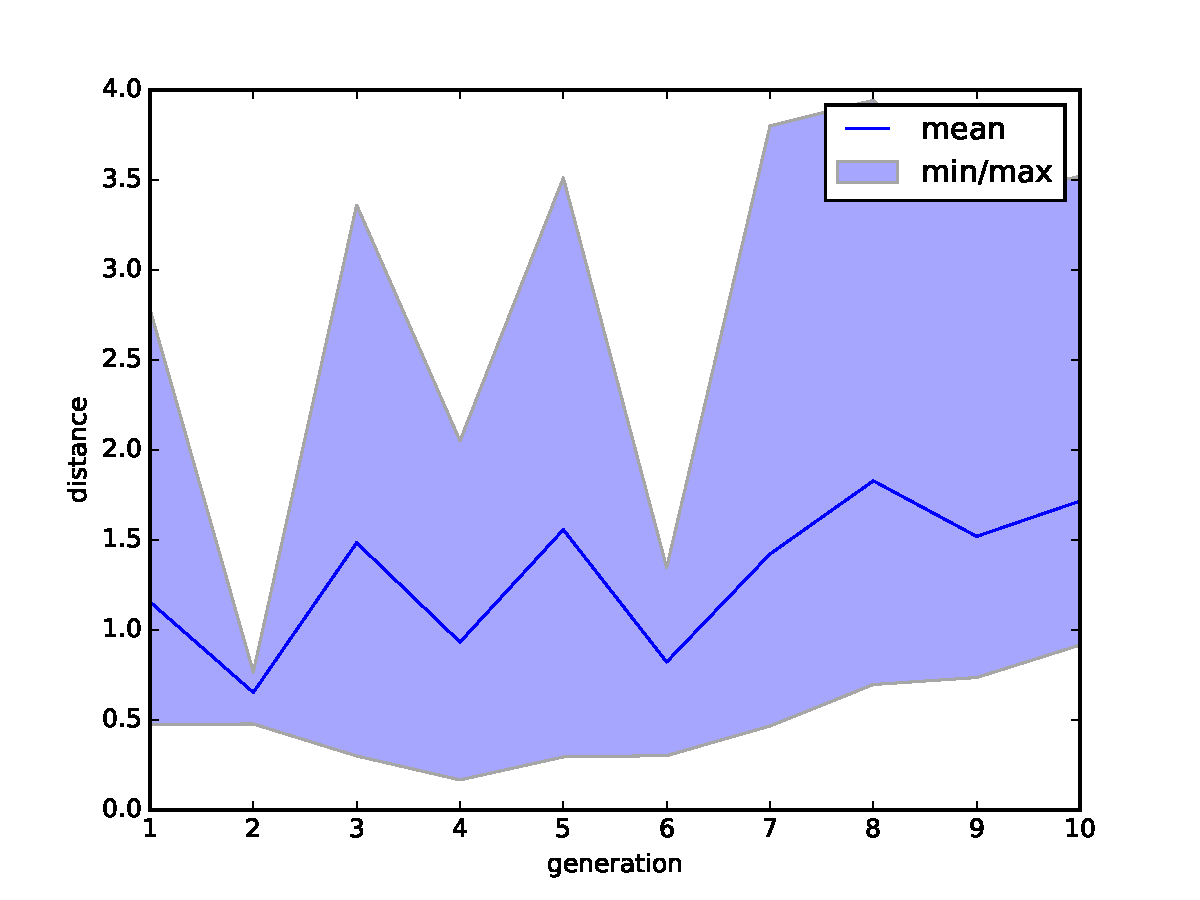
\includegraphics[width=\columnwidth]{figures/ea_plot.pdf}
\caption{10 generations with 6 individuals of the evolutionary algorithm.}
\label{fig:plot}
\end{figure}

The individuals of the evolutionary algorithm can execute throws, but due to glitches in the simulation, like the shaking and exploding hand (\autoref{fig:dispersed}), the measured distances are not representative for the quality of the movement.
In addition, the non-determinism in the simulation makes it even harder to compare the results as the same individual gets different distances when executed multiple times.
This can be observed by the dips in the maximum curve.
These issues result in the algorithm not really learning anything and evolving the weights rather randomly.
Finally, the crashing platform doesn't allow to run the algorithm for sufficient generations.